\documentclass[border=3pt,tikz]{standalone}
% Shared look for every TikZ figure in these notes.
% Included by each standalone figure file; also keeps the figures consistent
% with the colours used in the PDF and on the website.

\usepackage{tikz}
\usepackage{pgfplots}
\pgfplotsset{compat=1.18}
\usetikzlibrary{arrows.meta, decorations.markings, decorations.pathmorphing,
                patterns, calc, positioning}
\usepackage{amsmath}

% Series colours are the three validated categorical slots also used by the
% interactive widgets, so a path drawn in the printed notes and the same path on
% the website are the same colour. They clear the colour-vision-deficiency and
% contrast checks as a set; every path is direct-labelled as well, so colour is
% never the only thing carrying identity.
\definecolor{duPurple}{HTML}{68246D}
\definecolor{duBlue}{HTML}{2A78D6}
\definecolor{duRed}{HTML}{EB6834}
\definecolor{duGreen}{HTML}{1BAF7A}
\definecolor{duGrey}{HTML}{6B6B6B}

\tikzset{
  axisline/.style   = {-{Stealth[length=3mm]}, line width=0.7pt, black},
  path1/.style      = {duBlue,   line width=1.1pt},
  path2/.style      = {duRed,    line width=1.1pt},
  path3/.style      = {duGreen,  line width=1.1pt},
  statedot/.style   = {circle, fill=black, inner sep=1.4pt},
  arrowhead/.style  = {decoration={markings,
                        mark=at position #1 with {\arrow{Stealth[length=2.6mm]}}},
                       postaction={decorate}},
  lbl/.style        = {font=\small},
  slbl/.style       = {font=\footnotesize, duGrey},
  workfill/.style   = {duPurple, opacity=0.16},
}

\begin{document}
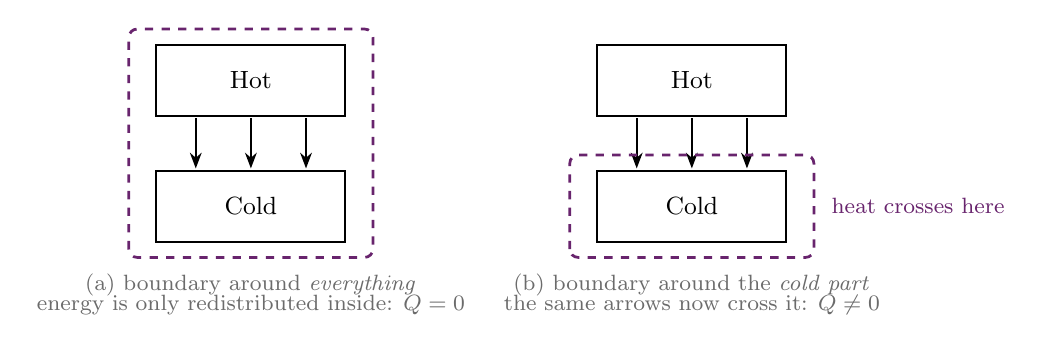
\begin{tikzpicture}[
  blk/.style   = {draw, line width=0.7pt, minimum width=24mm, minimum height=9mm, font=\small},
  bound/.style = {duPurple, dashed, line width=1pt, rounded corners=3pt},
]

% ---- (a) boundary around the whole block: Q = 0 --------------------------
\begin{scope}
  \node[blk] (h1) at (0,1.1) {Hot};
  \node[blk] (c1) at (0,-0.5) {Cold};
  \foreach \dx in {-0.7,0,0.7} {
    \draw[-{Stealth[length=2mm]}, line width=0.6pt] (\dx,0.62) -- (\dx,-0.02);
  }
  \draw[bound] (-1.55,-1.15) rectangle (1.55,1.75);
  \node[slbl, align=center] at (0,-1.62) {(a) boundary around \emph{everything}\\[-2pt]
    energy is only redistributed inside: $Q = 0$};
\end{scope}

% ---- (b) boundary around the cold part only: Q =/= 0 ---------------------
\begin{scope}[shift={(5.6,0)}]
  \node[blk] (h2) at (0,1.1) {Hot};
  \node[blk] (c2) at (0,-0.5) {Cold};
  \foreach \dx in {-0.7,0,0.7} {
    \draw[-{Stealth[length=2mm]}, line width=0.6pt] (\dx,0.62) -- (\dx,-0.02);
  }
  \draw[bound] (-1.55,-1.15) rectangle (1.55,0.15);
  \node[slbl, duPurple, right] at (1.65,-0.5) {heat crosses here};
  \node[slbl, align=center] at (0,-1.62) {(b) boundary around the \emph{cold part}\\[-2pt]
    the same arrows now cross it: $Q \neq 0$};
\end{scope}

\end{tikzpicture}
\end{document}
